\documentclass[t]{beamer}
\usefonttheme{serif}

\usepackage{amsmath,amsthm,amssymb,amsfonts,amscd,mathrsfs,amsxtra,multirow,kotex,mathtools,gensymb,textcomp,lipsum,tikz,verbatim,color,soul,courier,mdframed,xcolor}
\usepackage[normalem]{ulem}
\usetikzlibrary{calc,matrix,arrows,chains,positioning,scopes}
\usepackage{pdfpages}

\theoremstyle{plain}
\newtheorem{thm}{Theorem}[section]
\newtheorem{prop}[thm]{Proposition}

\theoremstyle{definition}
\newtheorem{defn}[thm]{Definition}
\newtheorem{exmp}[thm]{Example}
\newtheorem{excs}[thm]{Exercise}
\newtheorem{rem}[thm]{Remark}
\newtheorem{prob}[thm]{Problem}
\newtheorem{cor}[thm]{Corollary}

\newcommand \tr[1]{\textcolor{red}{#1}}
\newcommand{\tikzmark}[1]{\tikz[overlay,remember picture] \node (#1) {};}
\newcommand{\varep}{\varepsilon}
\newcommand{\DrawBox}[1][]{%
    \tikz[overlay,remember picture]{
    \draw[red,#1]
      ($(left)+(-0.2em,0.9em)$) rectangle
      ($(right)+(0.2em,-0.3em)$);}
}

\newcommand{\tikzmarkk}[2]{
    \tikz[overlay,remember picture,baseline] 
    \node[anchor=base] (#1) {$#2$};
}
\newcommand*\circled[1]{\tikz[baseline=(char.base)]{
            \node[shape=circle,draw,inner sep=2pt] (char) {#1};}}

\tikzset{join/.code=\tikzset{after node path={%
\ifx\tikzchainprevious\pgfutil@empty\else(\tikzchainprevious)%
edge[every join]#1(\tikzchaincurrent)\fi}}}

\tikzset{>=stealth',every on chain/.append style={join},
         every join/.style={->}}
\tikzstyle{labeled}=[execute at begin node=$\scriptstyle,
   execute at end node=$]

\newenvironment<>{proofs}[1][\proofname]{%
   \par
   \def\insertproofname{#1\@{.}}%
   \usebeamertemplate{proof begin}#2}
 {\usebeamertemplate{proof end}}
 

\addtobeamertemplate{navigation symbols}{}{%
    \usebeamerfont{footline}%
    \usebeamercolor[fg]{footline}%
    \hspace{1em}%
    \raisebox{2pt}[0pt][0pt]{\insertframenumber/\inserttotalframenumber}
}
\setbeamercolor{footline}{fg=blue}
\setbeamerfont{footline}{series=\bfseries}
\title[]{SE102:Multivariable Calculus}

\author[]{Hyosang Kang\inst{1}}

\institute[]{\inst{1}Division of Mathematics\\ School of Interdisciplinary Studies\\ DGIST}

\date[]{Lecture 05\\
Multiple Integrals}

\begin{document}

\begin{frame}
\titlepage
\end{frame}

\begin{frame}
\begin{defn}[Iterated integrals]
Let $f(x,y)$ be a two variable function define on a rectangular domain $D=[a,b]\times[c,d]$.
The \textbf{iterated integral} $\displaystyle \int_c^d\int_a^b f(x,y) dxdy$ on $D$ is defined as follows.
	$$\int_c^d\underbrace{\left[\int_a^b f(x,y)dx\right]}_{\textrm{consider $y$ as a constant}}dy.$$
\end{defn}
\begin{defn}[Double integral]
Let $f(x,y)$ be a function defined on a rectangular region $D=[a,b]\times[c,d]$.
Let us subdivide the intervals $[a,b]$ (respectively $[c,d]$) by $n$ ($m$, respectively) intervals.
	\[a=x_0<x_1<\cdots<x_n=b,\quad c=y_0<y_1<\cdots<y_m=d\]
\end{defn}
\end{frame}

\begin{frame}
The region $D$ is subdivided by $nm$ rectangular regions $D_{ij}=[x_{i-1},x_i]\times [y_{i-1},y_i]$.
For each $i=1,\cdots,n$ and $j =1,\cdots,m$, let us choose a point $(x_i^*,y_j^*)\in D_{ij}$.
Denote $\Delta x_i=x_{i}-x_{i-1}$, $\quad\Delta y_j=y_{j}-y_{j-1}$.
The sum 
	\[\sum_{i=1}^n\sum_{j=1}^mf(x_i^*,y_j^*)\Delta x_i\Delta y_j\]
is called the \textbf{Riemann sum} of $f(x,y)$ with respect to the subdivision $D_{ij}$'s.
If the limit exists when $n,m\to\infty$, we denote 
	\[\iint_DfdA=\lim\sum_{i=1}^n\sum_{j=1}^mf(x_i^*,y_i^*)\Delta x_i\Delta y_j\]
This is called the \textbf{double integral} of $f$ over $D$.
\end{frame}

\begin{frame}
\begin{thm}
If $f$ is continuous on the region $D=[a,b]\times[c,d]$, then the double integral $\displaystyle\iint_DfdA$ exists.
\end{thm}
\begin{exmp}
The function $\displaystyle f(x,y) = \frac{y}{1+xy}$ is continuous on $D=[0,1]\times[0,1]$.
Find the double integral $\displaystyle \iint_Dfdxdy$.
\end{exmp}
\begin{exmp}
Show that the function $f(x,y)$ on $[0,1]\times[0,1]$ defined by
	$$f(x,y)=\begin{dcases}
	1 & x\textrm{ or }y\textrm{ is rational}\\
	0 & \textrm{otherwise}
	\end{dcases}$$
is not integrable on $[0,1]\times[0,1]$.
\end{exmp}
\end{frame}

\begin{frame}
\begin{thm}[Fubini I]
Let $f(x,y)$ be a continuous function defined on $D=[a,b]\times[c,d]$.
Then
	\[\iint_DfdA = \int_a^b \int_c^df(x,y)dy dx = \int_c^d \int_a^bf(x,y)dx dy\]
\end{thm}
\begin{exmp} 
Compute
	\[\iint\displaylimits_{[0,1]\times[0,1]}\frac{y}{1+xy}dxdy\]
using Fubini's theorem.
\end{exmp}
\end{frame}

\begin{frame}
\begin{rem}
The \emph{continuity} condition in the theorem is crucial.
For example, let
	$$f(x,y)=\begin{dcases}
	\frac{x^2-y^2}{(x^2+y^2)^2}&(x,y)\neq(0,0)\\
	0&(x,y)=(0,0)
	\end{dcases}$$
Let us compute $\displaystyle\int_0^1\int_0^1f(x,y)dydx$ first.
	\begin{align*}
	\int_0^1\int_0^1\frac{x^2-y^2}{(x^2+y^2)^2}dydx &= \int_0^1 \frac{y}{x^2+y^2}\Big\vert_{y=0}^1dx \\
	&= \int_0^1 \frac{1}{1+x^2} dx = \tan^{-1}x\Big\vert_0^1 = \frac{\pi}{4}
    \end{align*}
\end{rem}
\end{frame}

\begin{frame}
Next, the iterated integral $\displaystyle\int_0^1\int_0^1f(x,y)dxdy$ is 
	\begin{align*}
	\int_0^1\int_0^1\frac{x^2-y^2}{(x^2+y^2)^2}dxdy &= \int_0^1 \frac{-x}{x^2+y^2}\Big\vert_{x=0}^1dx \\
	&= \int_0^1 \frac{-1}{1+y^2} dy = -\tan^{-1}y\Big\vert_0^1 = -\frac{\pi}{4}
	\end{align*}
and it does not coincide with $\displaystyle\int_0^1\int_0^1f(x,y)dydx$.
\end{frame}

\begin{frame}
\begin{defn}
Let $f(x,y)$ be defined on a \underline{bounded} region $D$ in $\mathbf R^2$.
Suppose that $D$ lies on a large rectangular domain, say $D\subset[a,b]\times[c,d]$. 
Let us define a new function $F(x,y)$ as follows.
    $$F(x,y)
    = \begin{dcases}
	f(x,y) & (x,y)\in D\\
	0 & (x,y)\notin D
	\end{dcases}$$
Then the \textbf{definite integral} of $f$ over the domain $D$ is defined as 
	\[\iint_Df(x,y)dxdy=\iint\displaylimits_{[a,b]\times[c,d]}F(x,y)dxdy\]
\end{defn}
\end{frame}

\begin{frame}
\begin{thm}[Fubini II]
Let  $f(x,y)$ be a continuous function defined on $D$.
If $D=\{(x,y)\,|\,a\le x\le b,\, g_1(x)\le y\le g_2(x)\}$,
then
	\[\iint_Df(x,y)dxdy=\int_a^b \int_{g_1(x)}^{g_2(x)}f(x,y)dy dx\]
Similarly, if $D=\{(x,y)\,|\,c\le y\le d,\, h_1(y)\le x\le h_2(y)\}$,
then
	\[\iint_Df(x,y)dxdy=\int_c^d \int_{h_1(y)}^{h_2(y)}f(x,y)dx dy\]
\end{thm}
\end{frame}

\begin{frame}
\begin{exmp} 
Let us compute $\displaystyle \iint_De^{-y^2}dxdy$ where $D$ is the triangular region whose vertices are
$(0,0)$, $(0,1)$, and $(1,1)$.
By Fubini's theorem,
	$$\iint_De^{-y^2}dxdy 
	= \int_0^1\left[\int_x^1 e^{-y^2}dy\right]dx
	= \int_0^1\left[\int_0^y e^{-y^2}dx\right]dy.$$
Find which integration works.
\end{exmp}
\end{frame}

\begin{frame}
\begin{defn}
Let $f(x,y,z)$ be a function defined on the boxed domain $D=[a,b]\times[c,d]\times[e,f]$.
The \textbf{triple integral} of $f(x,y,z)$ over $D$ is denoted by
	\[\iiint\displaylimits_{[a,b]\times[c,d]\times[e,f]}\mkern-18mu f(x,y,z)dxdydz\]
If $f$ is defined on a region $V\subset[a,b]\times[c,d]\times[e,f]$,
Then define
	$$F(x,y,z) = \begin{dcases}
	f(x,y,z) & \textrm{if }(x,y,z)\in V \\
	0 & \textrm{otherwise} \end{dcases}$$
Then the triple integral is defined as
	\[\iiint_Vf(x,y,z)dxdydz =\mkern-20mu \iiint\displaylimits_{[a,b]\times[c,d]\times[e,f]}\mkern-18mu F(x,y,z)dxdydz\]
\end{defn}
\end{frame}

\begin{frame}
\begin{thm}[Fubini III]
Let $f(x,y,z)$ be a continuous function defined on the region $V$.
	\[V=\{(x,y,z)\,|\,a\le x\le b,\,g_1(x)\le y\le g_2(x),\, h_1(x,y)\le z\le h_2(x,y)\}\]
Then the following holds.
	\[\iiint_Vf(x,y,z)dxdydz = \int_a^b \int_{g_1(x)}^{g_2(x)} \int_{h_1(x,y)}^{h_2(x,y)}f(x,y,z)dz dy dx\]
\end{thm}
\begin{figure}[h]
\begin{center}
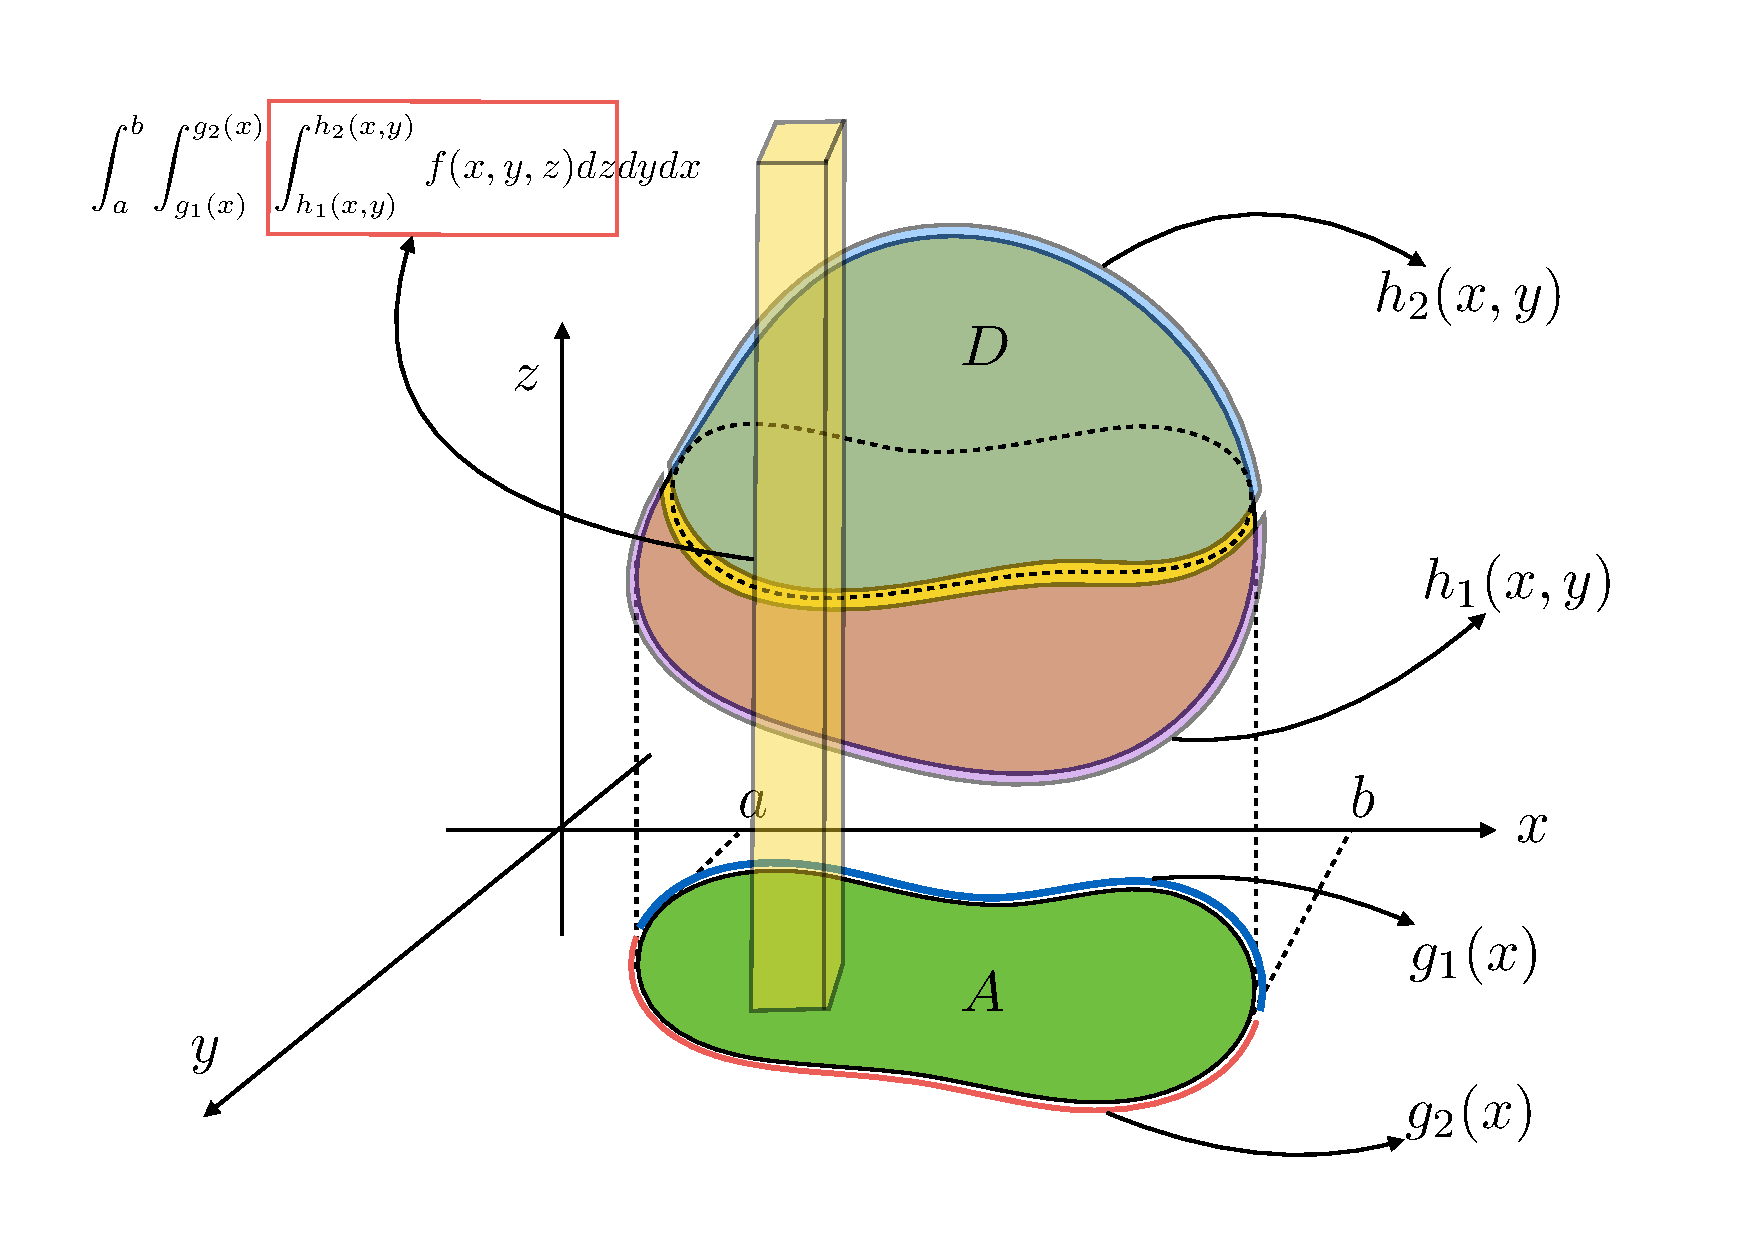
\includegraphics[scale=.2]{image/lnsec9-2}
\end{center}
\end{figure}
\end{frame}

\begin{frame}
\begin{exmp}
Let $V$ be a parallelopiped region bounded by $6$ planes : $2x=y$, $2x=y+2$, $y=0$, $y=4$, $z=0$, $z=3$.
Compute
	\[\iiint_V\frac{2x-y}{2}+\frac{z}{3}dxdydz\]
\end{exmp}
\end{frame}

\begin{frame}
\begin{defn}
Given an interval $I\subset\mathbf R$, a curve $C$ parametrized by $c:I\rightarrow\mathbf R^n$
	\[c(t)=(x_1(t),x_2(t),\cdots,x_n(t))\]
is \textbf{piecewise differentiable} if all coordinate function $x_i(t)$ are $\mathcal C^n$
on the interval $I$ except for finitely many points.
\end{defn}
\begin{defn}
Let $C$ be a piecewise differentiable curve on $\mathbf R^2$ parametrized by $c:[a,b]\to\mathbf R^2$.
Let $c'(t)=(x'(t),y'(t))$ be the velocity vector at the point $c(t)$.
Let $f(x,y)$ be a function defined on the curve $C$.
Then the \textbf{line integral} of $f(x,y)$ along $C$ is defined as
	\[\int_Cfds=\int_a^bf(c(t))|c'(t)|dt.\]
\end{defn}
\end{frame}

\begin{frame}
\begin{prop}
The line integral $\displaystyle \int_C f ds$ does not depend on the parametrization of $C$.
\end{prop}
\begin{proof}
Let $c:[a,b]\to\mathbf R^2$ be a parametrization of $C$.
Let $h:[c,d]\to[a,b]$ be a one-to-one correspondence which gives a \emph{re-parametrization} $c\circ h$ of $C$.
Let us write $t = h(\tau)$. Then
    \begin{align*}
        \int_c^df(c\circ h(\tau)) \cdot |(c\circ h)'(\tau)|d\tau 
        &= \int_c^d f(c(t)) \cdot |c'(t)| \cdot |h'(\tau)|d\tau \\
        &= \int_a^b f(c(t)) \cdot |c'(t)| dt
    \end{align*}
\end{proof}
\end{frame}

\begin{frame}
\begin{exmp}
Let us compute the line integral \[\displaystyle\int_C (2+x^2y)ds\]
where $C$ is the unit circle centered at the origin with counter clockwise orientation.
\end{exmp}
\end{frame}

\begin{frame}
\begin{defn}
Let $D$ be a region in $\mathbf R^2$ and $S$ a suface in $\mathbf R^3$.
A map $X:D\rightarrow S$
	\[X(u,v)=(x(u,v),y(u,v),z(u,v))\]
is called the \textbf{parametrization} of $S$ if
it is one-to-one correspondence and
every partial derivative of $x,y,z$ 
is continuous on $D$.
\end{defn}
\begin{exmp}
Find a parametrization of $x^2+y^2-z^2=1$.	
\end{exmp}
\end{frame}

\begin{frame}
\begin{defn}
Let $f(x,y,z)$ be a function defined on a surface $S$.
Let $X:D\rightarrow S$ be a parametrization of $S$.
The \textbf{surface integral} of $f$ on $S$ is defined by
	\begin{equation}\label{eqn-surf-int}
	\iint_SfdS=\iint_D(f\circ X)(u,v)\Vert X_u\times X_v\Vert dudv
	\end{equation}
\end{defn}

\begin{exmp}
Let $S$ be the surface defined by the graph of $z=\sqrt{x^2+y^2}$ over the disk $x^2+y^2\le 1$.
Evaluate 
	\[\iint_S zdS\]
\end{exmp}
\end{frame}

\begin{frame}
\begin{prob}
For $f(x,y) = x^2-y^2$, compute $\displaystyle \iint_S x+z dS$.
\end{prob}
\end{frame}

\begin{frame}
\begin{prob}
Let $f(x,y)$ is a density at the point $(x,y)$ on domain $D$.
Let
	$$\bar x= \frac{\iint_D xf(x,y)dA}{\iint_Df(x,y)dA},\quad 
	\bar y = \frac{\iint_D yf(x,y)dA}{\iint_Df(x,y)dA}$$
Explain why $(\bar x,\bar y)$ is the center of mass of $D$.
\end{prob}
\end{frame}

\begin{frame}
\begin{prob}
Let $V=\{0\le x\le 2,0\le y\le x,0\le z\le y\}$.
Write $\iiint_V f(x,y,z)$ in six different iterated integrals.
\end{prob}
\end{frame}

\begin{frame}
\begin{prob}
Let $f(x,y)$ be a function defined on a curve $C$.
Explain the meaning of the line integral $\int_Cfds$ in the following senses:
\begin{enumerate}
	\item when $f(x,y)$ is a density at $(x,y)$ on the curve $C$;
	\item the section of the graph $z=f(x,y)$ over the curve C.
\end{enumerate}
\end{prob}
\end{frame}
\end{document}